\documentclass[10pt,twocolumn]{article}
\usepackage[margin=0.75in]{geometry}
\usepackage[T1]{fontenc}
\usepackage[utf8]{inputenc}
\usepackage{lmodern}
\DeclareUnicodeCharacter{2295}{\ensuremath{\oplus}}
\DeclareUnicodeCharacter{00D7}{\ensuremath{\times}}
\DeclareUnicodeCharacter{00F7}{\ensuremath{\div}}
\DeclareUnicodeCharacter{2192}{\ensuremath{\to}}
\DeclareUnicodeCharacter{2264}{\ensuremath{\le}}
\usepackage{amsmath,amssymb}
\usepackage{booktabs}
\usepackage{graphicx}
\usepackage{xcolor}
\usepackage[numbers,sort&compress]{natbib}
\usepackage[colorlinks=true,linkcolor=blue!50!black,citecolor=blue!50!black,urlcolor=blue!50!black]{hyperref}
\usepackage{url}
\usepackage{enumitem}
\setlist{nosep,leftmargin=*}

% Small coloured change next to a score, as in Code2Video's tables. The colour says better or worse, not up or
% down: make_tables.delta() picks it from the column's direction (a drop on a lower-is-better column is \better),
% and columns with no better direction (sections rewritten, revisions used) get \neutral.
\definecolor{betterc}{HTML}{1F5FAD}\definecolor{worsec}{HTML}{C2491D}\definecolor{neutralc}{gray}{0.45}
\newcommand{\better}[1]{\,{\scriptsize\textcolor{betterc}{#1}}}
\newcommand{\worse}[1]{\,{\scriptsize\textcolor{worsec}{#1}}}
\newcommand{\neutral}[1]{\,{\scriptsize\textcolor{neutralc}{#1}}}
\newcommand{\hd}[1]{\begin{tabular}[b]{@{}c@{}}#1\end{tabular}}% a two-line table header

% A method figure generated from a prompt in figures/IMAGE_PROMPTS.md (Part A); a box names the prompt until the
% image file exists. Full text width in every document.
\newcommand{\paperfig}[4]{%
  \begin{figure*}[t]\centering
  \IfFileExists{figures/#1}{\includegraphics[width=\textwidth]{figures/#1}}{%
    \fbox{\parbox{0.92\textwidth}{\centering\small\vspace{22pt}\textit{Figure to generate: prompt #2 in}
    \texttt{paper/figures/IMAGE\_PROMPTS.md}, saved as \texttt{\detokenize{paper/figures/#1}}\vspace{22pt}}}}
  \caption{#3}\label{fig:#4}
  \end{figure*}}

% Every number below comes from paper/make_tables.py; a result that does not exist yet prints as [pending].
\newcommand{\pend}{\textcolor{red!70!black}{\textbf{[pending]}}}
\newcommand{\todo}[1]{\textcolor{red!70!black}{\textbf{[#1]}}}
\IfFileExists{tables/numbers.tex}{% generated by paper/make_tables.py; a missing macro means its result is pending
\newcommand{\AccGemmaBlind}{41.2}
\newcommand{\AccGemmaFixed}{70.0}
\newcommand{\AccGemmaFrames}{66.2}
\newcommand{\AccGemmaOther}{26.2}
\newcommand{\AccHaikuBlind}{53.1}
\newcommand{\AccHaikuFixed}{96.6}
\newcommand{\AccHaikuFrames}{98.1}
\newcommand{\AccHaikuOther}{42.5}
\newcommand{\AccSonnetBlind}{59.7}
\newcommand{\AccSonnetFixed}{82.2}
\newcommand{\AccSonnetFrames}{83.8}
\newcommand{\AccSonnetOther}{51.9}
\newcommand{\AdmClean}{5}
\newcommand{\AdmComplete}{10}
\newcommand{\AdmIncompleteBefore}{7}
\newcommand{\AdmRegenerated}{23}
\newcommand{\AdmTotal}{12}
\newcommand{\AllRuns}{282}
\newcommand{\AnsweredRight}{103}
\newcommand{\AnsweredRightShare}{100}
\newcommand{\AnsweredWithVideo}{103}
\newcommand{\AnsweredWrong}{0}
\newcommand{\ClaudeCost}{2.35}
\newcommand{\ClaudeCrowded}{7}
\newcommand{\ClaudeFaults}{96}
\newcommand{\ClaudeLeftover}{10}
\newcommand{\ClaudeOffScreen}{11}
\newcommand{\ClaudeOther}{22}
\newcommand{\ClaudeOverlap}{42}
\newcommand{\ClaudeSections}{40}
\newcommand{\ClaudeUnreadable}{4}
\newcommand{\FailedAttempts}{241}
\newcommand{\FirstTryFail}{42}
\newcommand{\LSAutoAttach}{13}
\newcommand{\LSAutoConflicts}{29}
\newcommand{\LSAutoFrames}{67.5}
\newcommand{\LSAutoMNine}{42.4}
\newcommand{\LSAutoMSeven}{18.5}
\newcommand{\LSAutoMvqs}{84.2}
\newcommand{\LSClaudeAttach}{4}
\newcommand{\LSClaudeConflicts}{4}
\newcommand{\LSClaudeFrames}{69.8}
\newcommand{\LSClaudeMNine}{47.6}
\newcommand{\LSClaudeMSeven}{19.1}
\newcommand{\LSClaudeMvqs}{85.6}
\newcommand{\LSDiff}{+5.1}
\newcommand{\LSDiffWithoutTop}{$-$1.3}
\newcommand{\LSGate}{not passed}
\newcommand{\LSLeftOut}{0}
\newcommand{\LSLosses}{5}
\newcommand{\LSN}{10}
\newcommand{\LSNeed}{7}
\newcommand{\LSOursAttach}{13}
\newcommand{\LSOursConflicts}{31}
\newcommand{\LSOursFrames}{67.5}
\newcommand{\LSOursMNine}{42.4}
\newcommand{\LSOursMSeven}{17.6}
\newcommand{\LSOursMvqs}{84.2}
\newcommand{\LSTopDiff}{+62.7}
\newcommand{\LSTopTopic}{Sorrel counts of lattice rectangles}
\newcommand{\LSWins}{5}
\newcommand{\LadMMMCAbstained}{89}
\newcommand{\LadMMMCAgreeEight}{--}
\newcommand{\LadMMMCAgreeNine}{--}
\newcommand{\LadMMMCAgreeOne}{0.94}
\newcommand{\LadMMMCAgreeRawNine}{0.87}
\newcommand{\LadMMMCAgreeRawSeven}{0.50}
\newcommand{\LadMMMCAgreeSeven}{--}
\newcommand{\LadMMMCAgreeThree}{--}
\newcommand{\LadMMMCAgreeTwo}{1.00}
\newcommand{\LadMMMCBlindAllRight}{12}
\newcommand{\LadMMMCDefinedEight}{0/12}
\newcommand{\LadMMMCDefinedNVG}{0/12}
\newcommand{\LadMMMCDefinedNine}{0/12}
\newcommand{\LadMMMCDefinedOne}{12/12}
\newcommand{\LadMMMCDefinedRawNine}{12/12}
\newcommand{\LadMMMCDefinedRawSeven}{12/12}
\newcommand{\LadMMMCDefinedSeven}{0/12}
\newcommand{\LadMMMCDefinedThree}{0/12}
\newcommand{\LadMMMCDefinedTwo}{12/12}
\newcommand{\LadMMMCLAEight}{--}
\newcommand{\LadMMMCLANine}{--}
\newcommand{\LadMMMCLAOne}{+0.6}
\newcommand{\LadMMMCLARawNine}{+0.1}
\newcommand{\LadMMMCLARawSeven}{+0.3}
\newcommand{\LadMMMCLASeven}{--}
\newcommand{\LadMMMCLAThree}{--}
\newcommand{\LadMMMCLATwo}{0.0}
\newcommand{\LadMMMCLBEight}{--}
\newcommand{\LadMMMCLBNine}{--}
\newcommand{\LadMMMCLBOne}{+7.2}
\newcommand{\LadMMMCLBRawNine}{+0.1}
\newcommand{\LadMMMCLBRawSeven}{+1.4}
\newcommand{\LadMMMCLBSeven}{--}
\newcommand{\LadMMMCLBThree}{--}
\newcommand{\LadMMMCLBTwo}{0.0}
\newcommand{\LadMMMCLGEight}{--}
\newcommand{\LadMMMCLGNine}{--}
\newcommand{\LadMMMCLGOne}{+2.8}
\newcommand{\LadMMMCLGRawNine}{0.0}
\newcommand{\LadMMMCLGRawSeven}{$-$0.1}
\newcommand{\LadMMMCLGSeven}{--}
\newcommand{\LadMMMCLGThree}{--}
\newcommand{\LadMMMCLGTwo}{0.0}
\newcommand{\LadMMMCSBlind}{100.0}
\newcommand{\LadMMMCSFrames}{98.2}
\newcommand{\LadMMMCSStatic}{99.5}
\newcommand{\LadMMMCSVisual}{98.4}
\newcommand{\LadMMMCSepEight}{--}
\newcommand{\LadMMMCSepNine}{--}
\newcommand{\LadMMMCSepOne}{+10.6}
\newcommand{\LadMMMCSepRawNine}{+13.0}
\newcommand{\LadMMMCSepRawSeven}{+4.1}
\newcommand{\LadMMMCSepSeven}{--}
\newcommand{\LadMMMCSepThree}{--}
\newcommand{\LadMMMCSepTwo}{+16.7}
\newcommand{\LadMMMCTiesEight}{--}
\newcommand{\LadMMMCTiesNine}{--}
\newcommand{\LadMMMCTiesOne}{7}
\newcommand{\LadMMMCTiesRawNine}{0}
\newcommand{\LadMMMCTiesRawSeven}{1}
\newcommand{\LadMMMCTiesSeven}{--}
\newcommand{\LadMMMCTiesThree}{--}
\newcommand{\LadMMMCTiesTwo}{12}
\newcommand{\LadMMMCTopics}{12}
\newcommand{\LadMMMCVideos}{48}
\newcommand{\LadNovelAbstained}{42}
\newcommand{\LadNovelAgreeEight}{--}
\newcommand{\LadNovelAgreeNine}{--}
\newcommand{\LadNovelAgreeOne}{0.67}
\newcommand{\LadNovelAgreeRawNine}{0.30}
\newcommand{\LadNovelAgreeRawSeven}{-0.32}
\newcommand{\LadNovelAgreeSeven}{--}
\newcommand{\LadNovelAgreeThree}{0.43}
\newcommand{\LadNovelAgreeTwo}{0.21}
\newcommand{\LadNovelBlindAllRight}{0}
\newcommand{\LadNovelDefinedEight}{10/10}
\newcommand{\LadNovelDefinedNVG}{10/10}
\newcommand{\LadNovelDefinedNine}{10/10}
\newcommand{\LadNovelDefinedOne}{10/10}
\newcommand{\LadNovelDefinedRawNine}{10/10}
\newcommand{\LadNovelDefinedRawSeven}{10/10}
\newcommand{\LadNovelDefinedSeven}{10/10}
\newcommand{\LadNovelDefinedThree}{10/10}
\newcommand{\LadNovelDefinedTwo}{10/10}
\newcommand{\LadNovelLAEight}{+9.6}
\newcommand{\LadNovelLANine}{+9.6}
\newcommand{\LadNovelLAOne}{+11.7}
\newcommand{\LadNovelLARawNine}{+4.6}
\newcommand{\LadNovelLARawSeven}{$-$2.0}
\newcommand{\LadNovelLASeven}{$-$1.4}
\newcommand{\LadNovelLAThree}{+7.0}
\newcommand{\LadNovelLATwo}{+3.8}
\newcommand{\LadNovelLBEight}{+9.8}
\newcommand{\LadNovelLBNine}{+6.1}
\newcommand{\LadNovelLBOne}{$-$2.9}
\newcommand{\LadNovelLBRawNine}{+2.0}
\newcommand{\LadNovelLBRawSeven}{+0.7}
\newcommand{\LadNovelLBSeven}{$-$0.5}
\newcommand{\LadNovelLBThree}{+6.8}
\newcommand{\LadNovelLBTwo}{+3.8}
\newcommand{\LadNovelLGEight}{+8.0}
\newcommand{\LadNovelLGNine}{+6.1}
\newcommand{\LadNovelLGOne}{+1.7}
\newcommand{\LadNovelLGRawNine}{+2.7}
\newcommand{\LadNovelLGRawSeven}{+1.9}
\newcommand{\LadNovelLGSeven}{+3.4}
\newcommand{\LadNovelLGThree}{+5.5}
\newcommand{\LadNovelLGTwo}{+3.8}
\newcommand{\LadNovelSBlind}{41.0}
\newcommand{\LadNovelSFrames}{67.5}
\newcommand{\LadNovelSStatic}{47.2}
\newcommand{\LadNovelSVisual}{49.8}
\newcommand{\LadNovelSepEight}{+26.1}
\newcommand{\LadNovelSepNine}{+64.4}
\newcommand{\LadNovelSepOne}{+48.3}
\newcommand{\LadNovelSepRawNine}{+36.3}
\newcommand{\LadNovelSepRawSeven}{+11.7}
\newcommand{\LadNovelSepSeven}{+25.8}
\newcommand{\LadNovelSepThree}{+74.5}
\newcommand{\LadNovelSepTwo}{+42.5}
\newcommand{\LadNovelTiesEight}{0}
\newcommand{\LadNovelTiesNine}{0}
\newcommand{\LadNovelTiesOne}{0}
\newcommand{\LadNovelTiesRawNine}{0}
\newcommand{\LadNovelTiesRawSeven}{0}
\newcommand{\LadNovelTiesSeven}{0}
\newcommand{\LadNovelTiesThree}{4}
\newcommand{\LadNovelTiesTwo}{4}
\newcommand{\LadNovelTopics}{10}
\newcommand{\LadNovelVideos}{40}
\newcommand{\LadSmallAbstained}{--}
\newcommand{\LadSmallAgreeEight}{--}
\newcommand{\LadSmallAgreeNine}{--}
\newcommand{\LadSmallAgreeOne}{--}
\newcommand{\LadSmallAgreeRawNine}{0.32}
\newcommand{\LadSmallAgreeRawSeven}{--}
\newcommand{\LadSmallAgreeSeven}{--}
\newcommand{\LadSmallAgreeThree}{0.82}
\newcommand{\LadSmallAgreeTwo}{0.57}
\newcommand{\LadSmallBlindAllRight}{6}
\newcommand{\LadSmallDefinedEight}{0/12}
\newcommand{\LadSmallDefinedNVG}{6/12}
\newcommand{\LadSmallDefinedNine}{9/12}
\newcommand{\LadSmallDefinedOne}{0/12}
\newcommand{\LadSmallDefinedRawNine}{12/12}
\newcommand{\LadSmallDefinedRawSeven}{0/12}
\newcommand{\LadSmallDefinedSeven}{0/12}
\newcommand{\LadSmallDefinedThree}{6/12}
\newcommand{\LadSmallDefinedTwo}{12/12}
\newcommand{\LadSmallLAEight}{--}
\newcommand{\LadSmallLANine}{+5.9}
\newcommand{\LadSmallLAOne}{--}
\newcommand{\LadSmallLARawNine}{+1.2}
\newcommand{\LadSmallLARawSeven}{--}
\newcommand{\LadSmallLASeven}{--}
\newcommand{\LadSmallLAThree}{+16.7}
\newcommand{\LadSmallLATwo}{+3.3}
\newcommand{\LadSmallLBEight}{--}
\newcommand{\LadSmallLBNine}{$-$23.7}
\newcommand{\LadSmallLBOne}{--}
\newcommand{\LadSmallLBRawNine}{$-$2.9}
\newcommand{\LadSmallLBRawSeven}{--}
\newcommand{\LadSmallLBSeven}{--}
\newcommand{\LadSmallLBThree}{+25.0}
\newcommand{\LadSmallLBTwo}{$-$3.3}
\newcommand{\LadSmallLGEight}{--}
\newcommand{\LadSmallLGNine}{$-$0.6}
\newcommand{\LadSmallLGOne}{--}
\newcommand{\LadSmallLGRawNine}{+0.2}
\newcommand{\LadSmallLGRawSeven}{--}
\newcommand{\LadSmallLGSeven}{--}
\newcommand{\LadSmallLGThree}{+8.3}
\newcommand{\LadSmallLGTwo}{+1.7}
\newcommand{\LadSmallSBlind}{81.7}
\newcommand{\LadSmallSFrames}{79.5}
\newcommand{\LadSmallSepEight}{--}
\newcommand{\LadSmallSepNine}{+37.9}
\newcommand{\LadSmallSepOne}{--}
\newcommand{\LadSmallSepRawNine}{+6.4}
\newcommand{\LadSmallSepRawSeven}{--}
\newcommand{\LadSmallSepSeven}{--}
\newcommand{\LadSmallSepThree}{+16.7}
\newcommand{\LadSmallSepTwo}{+10.0}
\newcommand{\LadSmallTiesEight}{--}
\newcommand{\LadSmallTiesNine}{1}
\newcommand{\LadSmallTiesOne}{--}
\newcommand{\LadSmallTiesRawNine}{1}
\newcommand{\LadSmallTiesRawSeven}{--}
\newcommand{\LadSmallTiesSeven}{--}
\newcommand{\LadSmallTiesThree}{4}
\newcommand{\LadSmallTiesTwo}{9}
\newcommand{\LadSmallTopics}{12}
\newcommand{\LadSmallVideos}{48}
\newcommand{\NMCount}{+9.6}
\newcommand{\NMCountMDE}{42.6}
\newcommand{\NMCountN}{10}
\newcommand{\NMCountP}{0.221}
\newcommand{\NMCountPTopics}{0.377}
\newcommand{\NMCountPos}{6}
\newcommand{\NMDense}{+14.1}
\newcommand{\NMDenseMDE}{28.0}
\newcommand{\NMDenseN}{10}
\newcommand{\NMDenseP}{0.050}
\newcommand{\NMDensePTopics}{0.016}
\newcommand{\NMDensePos}{9}
\newcommand{\NMFloorAll}{1.9}
\newcommand{\NMFloorOne}{7.2}
\newcommand{\NMFramesDense}{+28.4}
\newcommand{\NMFramesDenseMDE}{37.7}
\newcommand{\NMFramesDenseN}{10}
\newcommand{\NMFramesDenseP}{0.002}
\newcommand{\NMFramesDensePTopics}{0.014}
\newcommand{\NMFramesDensePos}{8}
\newcommand{\NMGain}{+42.4}
\newcommand{\NMGainMDE}{39.4}
\newcommand{\NMGainN}{10}
\newcommand{\NMGainP}{0.000}
\newcommand{\NMGainPTopics}{0.008}
\newcommand{\NMGainPos}{9}
\newcommand{\NMHGain}{+89.2}
\newcommand{\NMHGainMDE}{30.8}
\newcommand{\NMHGainN}{10}
\newcommand{\NMHGainP}{0.000}
\newcommand{\NMHGainPTopics}{0.004}
\newcommand{\NMHGainPos}{9}
\newcommand{\NMHLayout}{$-$1.5}
\newcommand{\NMHLayoutMDE}{22.3}
\newcommand{\NMHLayoutN}{10}
\newcommand{\NMHLayoutP}{0.777}
\newcommand{\NMHLayoutPTopics}{0.875}
\newcommand{\NMHLayoutPos}{2}
\newcommand{\NMHRepChanged}{8}
\newcommand{\NMHRepN}{320}
\newcommand{\NMHSpec}{+150.6}
\newcommand{\NMHSpecMDE}{95.7}
\newcommand{\NMHSpecN}{10}
\newcommand{\NMHSpecP}{0.000}
\newcommand{\NMHSpecPTopics}{0.002}
\newcommand{\NMHSpecPos}{10}
\newcommand{\NMLayout}{+5.1}
\newcommand{\NMLayoutMDE}{24.2}
\newcommand{\NMLayoutN}{10}
\newcommand{\NMLayoutP}{0.266}
\newcommand{\NMLayoutPTopics}{0.619}
\newcommand{\NMLayoutPos}{5}
\newcommand{\NMRepair}{+6.1}
\newcommand{\NMRepairGeneric}{+6.1}
\newcommand{\NMRepairGenericMDE}{29.9}
\newcommand{\NMRepairGenericN}{10}
\newcommand{\NMRepairGenericP}{0.392}
\newcommand{\NMRepairGenericPTopics}{0.449}
\newcommand{\NMRepairGenericPos}{6}
\newcommand{\NMRepairMDE}{29.5}
\newcommand{\NMRepairN}{10}
\newcommand{\NMRepairP}{0.356}
\newcommand{\NMRepairPTopics}{0.453}
\newcommand{\NMRepairPos}{6}
\newcommand{\NMRepeatMoved}{33}
\newcommand{\NMRepeatN}{232}
\newcommand{\NMRuleFPR}{8.2}
\newcommand{\NMSGain}{+45.9}
\newcommand{\NMSGainMDE}{47.7}
\newcommand{\NMSGainN}{10}
\newcommand{\NMSGainP}{0.001}
\newcommand{\NMSGainPTopics}{0.012}
\newcommand{\NMSGainPos}{8}
\newcommand{\NMSLayout}{$-$16.3}
\newcommand{\NMSLayoutMDE}{49.3}
\newcommand{\NMSLayoutN}{10}
\newcommand{\NMSLayoutP}{0.080}
\newcommand{\NMSLayoutPTopics}{0.539}
\newcommand{\NMSLayoutPos}{4}
\newcommand{\NMSRepChanged}{10}
\newcommand{\NMSRepN}{320}
\newcommand{\NMSSpec}{+90.8}
\newcommand{\NMSSpecMDE}{70.6}
\newcommand{\NMSSpecN}{10}
\newcommand{\NMSSpecP}{0.000}
\newcommand{\NMSSpecPTopics}{0.002}
\newcommand{\NMSSpecPos}{10}
\newcommand{\NMSize}{+18.8}
\newcommand{\NMSizeMDE}{37.2}
\newcommand{\NMSizeN}{10}
\newcommand{\NMSizeP}{0.008}
\newcommand{\NMSizePTopics}{0.033}
\newcommand{\NMSizePos}{6}
\newcommand{\NMSmall}{$-$23.7}
\newcommand{\NMSmallMDE}{160.2}
\newcommand{\NMSmallN}{9}
\newcommand{\NMSmallP}{0.223}
\newcommand{\NMSmallPTopics}{0.727}
\newcommand{\NMSmallPos}{5}
\newcommand{\NMSpec}{+64.4}
\newcommand{\NMSpecMDE}{42.7}
\newcommand{\NMSpecN}{10}
\newcommand{\NMSpecP}{0.000}
\newcommand{\NMSpecPTopics}{0.002}
\newcommand{\NMSpecPos}{10}
\newcommand{\NMStageFive}{+6.0}
\newcommand{\NMStageFiveGeneric}{+6.3}
\newcommand{\NMStageFiveGenericMDE}{11.6}
\newcommand{\NMStageFiveGenericN}{10}
\newcommand{\NMStageFiveGenericP}{0.015}
\newcommand{\NMStageFiveGenericPTopics}{0.062}
\newcommand{\NMStageFiveGenericPos}{5}
\newcommand{\NMStageFiveMDE}{11.7}
\newcommand{\NMStageFiveN}{10}
\newcommand{\NMStageFiveP}{0.023}
\newcommand{\NMStageFivePTopics}{0.125}
\newcommand{\NMStageFivePos}{4}
\newcommand{\NMStageFour}{+2.5}
\newcommand{\NMStageFourGeneric}{+2.0}
\newcommand{\NMStageFourGenericMDE}{6.5}
\newcommand{\NMStageFourGenericN}{10}
\newcommand{\NMStageFourGenericP}{0.268}
\newcommand{\NMStageFourGenericPTopics}{0.375}
\newcommand{\NMStageFourGenericPos}{3}
\newcommand{\NMStageFourMDE}{5.6}
\newcommand{\NMStageFourN}{10}
\newcommand{\NMStageFourP}{0.101}
\newcommand{\NMStageFourPTopics}{0.250}
\newcommand{\NMStageFourPos}{3}
\newcommand{\NMStageOne}{+7.7}
\newcommand{\NMStageOneGeneric}{+5.6}
\newcommand{\NMStageOneGenericMDE}{22.4}
\newcommand{\NMStageOneGenericN}{10}
\newcommand{\NMStageOneGenericP}{0.325}
\newcommand{\NMStageOneGenericPTopics}{0.328}
\newcommand{\NMStageOneGenericPos}{4}
\newcommand{\NMStageOneMDE}{21.7}
\newcommand{\NMStageOneN}{10}
\newcommand{\NMStageOneP}{0.132}
\newcommand{\NMStageOnePTopics}{0.125}
\newcommand{\NMStageOnePos}{4}
\newcommand{\NMStageThree}{+3.4}
\newcommand{\NMStageThreeGeneric}{+2.1}
\newcommand{\NMStageThreeGenericMDE}{11.8}
\newcommand{\NMStageThreeGenericN}{10}
\newcommand{\NMStageThreeGenericP}{0.564}
\newcommand{\NMStageThreeGenericPTopics}{0.875}
\newcommand{\NMStageThreeGenericPos}{2}
\newcommand{\NMStageThreeMDE}{11.0}
\newcommand{\NMStageThreeN}{10}
\newcommand{\NMStageThreeP}{0.008}
\newcommand{\NMStageThreePTopics}{1.000}
\newcommand{\NMStageThreePos}{1}
\newcommand{\NMStageTwo}{+12.2}
\newcommand{\NMStageTwoGeneric}{+3.4}
\newcommand{\NMStageTwoGenericMDE}{11.4}
\newcommand{\NMStageTwoGenericN}{10}
\newcommand{\NMStageTwoGenericP}{0.171}
\newcommand{\NMStageTwoGenericPTopics}{0.344}
\newcommand{\NMStageTwoGenericPos}{4}
\newcommand{\NMStageTwoMDE}{23.7}
\newcommand{\NMStageTwoN}{10}
\newcommand{\NMStageTwoP}{0.017}
\newcommand{\NMStageTwoPTopics}{0.125}
\newcommand{\NMStageTwoPos}{4}
\newcommand{\NovelItems}{96}
\newcommand{\NovelUnknown}{58}
\newcommand{\NullNoVideo}{100}
\newcommand{\NullWithVideo}{85}
\newcommand{\NullWithVideoN}{602}
\newcommand{\OrderRuns}{146}
\newcommand{\OrderShare}{52}
\newcommand{\PilotDev}{127}
\newcommand{\PilotDevGain}{+12.2}
\newcommand{\PilotFlagged}{3.3}
\newcommand{\PilotGaps}{124}
\newcommand{\PilotLayoutAll}{72.6}
\newcommand{\PilotLayoutBase}{78.5}
\newcommand{\PilotNotKept}{9}
\newcommand{\PilotRevisions}{36}
\newcommand{\PilotSections}{4}
\newcommand{\PilotTies}{7}
\newcommand{\PreflightFP}{1}
\newcommand{\PreflightN}{156}
\newcommand{\ShiftNotes}{25}
\newcommand{\ShiftsIn}{41}
\newcommand{\ShiftsRemoved}{38}
\newcommand{\SyntaxAfterPatch}{38}
\newcommand{\mmmcpriorGemmaAcc}{99.0}
\newcommand{\mmmcpriorGemmaAllRight}{108}
\newcommand{\mmmcpriorGemmaP}{99.0}
\newcommand{\mmmcpriorGemmaTopics}{117}
\newcommand{\mmmcpriorQwenAcc}{97.4}
\newcommand{\mmmcpriorQwenAllRight}{99}
\newcommand{\mmmcpriorQwenP}{95.6}
\newcommand{\mmmcpriorQwenSmallAcc}{91.9}
\newcommand{\mmmcpriorQwenSmallAllRight}{67}
\newcommand{\mmmcpriorQwenSmallP}{86.6}
\newcommand{\mmmcpriorQwenSmallTopics}{117}
\newcommand{\mmmcpriorQwenTopics}{117}
\newcommand{\novelcardGemmaAcc}{84.9}
\newcommand{\novelcardGemmaAllRight}{1}
\newcommand{\novelcardGemmaP}{83.7}
\newcommand{\novelcardGemmaTopics}{12}
\newcommand{\novelpriorGemmaAcc}{41.1}
\newcommand{\novelpriorGemmaAllRight}{0}
\newcommand{\novelpriorGemmaP}{41.4}
\newcommand{\novelpriorGemmaTopics}{12}
}{}
\providecommand{\AllRuns}{\pend}\providecommand{\OrderRuns}{\pend}\providecommand{\OrderShare}{\pend}
\providecommand{\NullWithVideo}{\pend}\providecommand{\NullNoVideo}{\pend}\providecommand{\PilotTies}{\pend}
\providecommand{\FailedAttempts}{\pend}\providecommand{\FirstTryFail}{\pend}
\providecommand{\PreflightFP}{\pend}\providecommand{\PilotNotKept}{\pend}\providecommand{\PilotRevisions}{\pend}\providecommand{\PreflightN}{\pend}\providecommand{\SyntaxAfterPatch}{\pend}\providecommand{\PilotGaps}{\pend}\providecommand{\PilotDev}{\pend}\providecommand{\PilotFlagged}{\pend}\providecommand{\PilotSections}{\pend}\providecommand{\PilotDevGain}{\pend}
\providecommand{\mmmcpriorGemmaAcc}{\pend}\providecommand{\mmmcpriorGemmaP}{\pend}
\providecommand{\mmmcpriorGemmaAllRight}{\pend}\providecommand{\mmmcpriorGemmaTopics}{\pend}
\providecommand{\mmmcpriorQwenAcc}{\pend}\providecommand{\mmmcpriorQwenSmallAcc}{\pend}\providecommand{\mmmcpriorQwenP}{\pend}
\providecommand{\novelpriorGemmaAcc}{\pend}\providecommand{\novelpriorGemmaP}{\pend}
\providecommand{\novelcardGemmaAcc}{\pend}\providecommand{\novelcardGemmaP}{\pend}
\providecommand{\LadMMMCBlindAllRight}{\pend}\providecommand{\LadMMMCTopics}{\pend}\providecommand{\LadMMMCAbstained}{\pend}
\providecommand{\LadMMMCVideos}{\pend}\providecommand{\LadMMMCSepOne}{\pend}\providecommand{\LadMMMCSepTwo}{\pend}\providecommand{\LadMMMCLBOne}{\pend}\providecommand{\LadMMMCLBTwo}{\pend}\providecommand{\LadMMMCTiesOne}{\pend}\providecommand{\LadMMMCTiesTwo}{\pend}\providecommand{\LadMMMCDefinedNVG}{\pend}
\providecommand{\LadSmallSBlind}{\pend}\providecommand{\LadSmallDefinedNine}{\pend}\providecommand{\LadSmallSepNine}{\pend}\providecommand{\LadSmallSepRawNine}{\pend}\providecommand{\LadSmallLBNine}{\pend}\providecommand{\LadSmallLBRawNine}{\pend}\providecommand{\LadSmallLGNine}{\pend}\providecommand{\LadMMMCSBlind}{\pend}\providecommand{\LadMMMCSVisual}{\pend}\providecommand{\LadMMMCSepRawNine}{\pend}
\providecommand{\LadNovelSBlind}{\pend}\providecommand{\LadNovelDefinedNine}{\pend}\providecommand{\LadNovelSepNine}{\pend}\providecommand{\LadNovelDefinedSeven}{\pend}\providecommand{\LadNovelSepSeven}{\pend}\providecommand{\LadNovelSFrames}{\pend}\providecommand{\LadNovelSVisual}{\pend}\providecommand{\AdmIncompleteBefore}{\pend}\providecommand{\AdmTotal}{\pend}\providecommand{\AdmComplete}{\pend}\providecommand{\AdmClean}{\pend}\providecommand{\ClaudeFaults}{\pend}\providecommand{\ClaudeSections}{\pend}\providecommand{\ClaudeCost}{\pend}\providecommand{\ClaudeOverlap}{\pend}\providecommand{\ClaudeOther}{\pend}\providecommand{\ClaudeOffScreen}{\pend}\providecommand{\ClaudeLeftover}{\pend}\providecommand{\ClaudeCrowded}{\pend}\providecommand{\ClaudeUnreadable}{\pend}\providecommand{\ShiftsIn}{\pend}\providecommand{\ShiftsRemoved}{\pend}\providecommand{\ShiftNotes}{\pend}\providecommand{\LSDiff}{\pend}\providecommand{\LSWins}{\pend}\providecommand{\LSN}{\pend}\providecommand{\LSGate}{\pend}
\providecommand{\LadNovelBlindAllRight}{\pend}\providecommand{\LadNovelTopics}{\pend}\providecommand{\LadNovelAbstained}{\pend}

\newcommand{\Sblind}{S_{\text{none}}}
\newcommand{\Sstatic}{S_{\text{static}}}
\newcommand{\Svisual}{S_{\text{visual}}}
\newcommand{\Beff}{B_{\text{eff}}}
% noise model (bench/noise_model.py), filled by make_tables.py
\providecommand{\LSOursConflicts}{\pend}\providecommand{\LSClaudeConflicts}{\pend}\providecommand{\LSOursAttach}{\pend}\providecommand{\LSClaudeAttach}{\pend}\providecommand{\LSOursMvqs}{\pend}\providecommand{\LSClaudeMvqs}{\pend}\providecommand{\NMRepeatMoved}{\pend}\providecommand{\NMRepeatN}{\pend}\providecommand{\NMFloorOne}{\pend}\providecommand{\NMFloorAll}{\pend}\providecommand{\NMGain}{\pend}\providecommand{\NMGainPos}{\pend}\providecommand{\NMGainN}{\pend}\providecommand{\NMSpec}{\pend}\providecommand{\NMSpecPos}{\pend}\providecommand{\NMSpecN}{\pend}\providecommand{\NMFramesDense}{\pend}\providecommand{\NMFramesDensePos}{\pend}\providecommand{\NMFramesDenseN}{\pend}\providecommand{\NMLayoutMDE}{\pend}\providecommand{\NMRuleFPR}{\pend}\providecommand{\NMSmallMDE}{\pend}
\providecommand{\NMSize}{\pend}\providecommand{\NMSizePos}{\pend}\providecommand{\NMSizeN}{\pend}\providecommand{\NMCount}{\pend}\providecommand{\NMHGain}{\pend}\providecommand{\NMHGainPos}{\pend}\providecommand{\NMHGainN}{\pend}\providecommand{\NMSGain}{\pend}\providecommand{\NMSGainPos}{\pend}\providecommand{\NMSGainN}{\pend}\providecommand{\NMHSpecPos}{\pend}\providecommand{\NMHSpecN}{\pend}\providecommand{\NMSSpecPos}{\pend}\providecommand{\NMSSpecN}{\pend}\providecommand{\NMHLayout}{\pend}\providecommand{\NMSLayout}{\pend}\providecommand{\NMHRepChanged}{\pend}\providecommand{\NMHRepN}{\pend}\providecommand{\NMSRepChanged}{\pend}\providecommand{\AccHaikuBlind}{\pend}\providecommand{\AccSonnetBlind}{\pend}\providecommand{\AccGemmaBlind}{\pend}\providecommand{\AccHaikuFrames}{\pend}\providecommand{\AccSonnetFrames}{\pend}
\providecommand{\NMRepair}{\pend}\providecommand{\NMRepairPos}{\pend}\providecommand{\NMRepairN}{\pend}\providecommand{\NMRepairMDE}{\pend}\providecommand{\NMRepairGeneric}{\pend}\providecommand{\NMRepairGenericPos}{\pend}\providecommand{\NMRepairGenericN}{\pend}\providecommand{\NMRepairGenericMDE}{\pend}

% Let tall tables sit at the top of a text page instead of waiting for a float page (LaTeX's defaults allow 70%
% and push every later table behind the first one that does not fit, to the end of the document).
\renewcommand{\topfraction}{0.9}\renewcommand{\bottomfraction}{0.8}\renewcommand{\textfraction}{0.07}
\renewcommand{\floatpagefraction}{0.8}\renewcommand{\dbltopfraction}{0.9}\renewcommand{\dblfloatpagefraction}{0.8}
\setcounter{topnumber}{3}\setcounter{bottomnumber}{2}\setcounter{totalnumber}{5}\setcounter{dbltopnumber}{3}
\providecommand{\NMStageOne}{\pend}\providecommand{\NMStageOnePos}{\pend}\providecommand{\NMStageOneN}{\pend}\providecommand{\NMStageOneMDE}{\pend}\providecommand{\NMStageOneP}{\pend}\providecommand{\NMStageOnePTopics}{\pend}\providecommand{\NMStageOneGeneric}{\pend}\providecommand{\NMStageOneGenericPos}{\pend}\providecommand{\NMStageOneGenericN}{\pend}\providecommand{\NMStageOneGenericMDE}{\pend}\providecommand{\NMStageOneGenericP}{\pend}\providecommand{\NMStageOneGenericPTopics}{\pend}\providecommand{\NMStageTwo}{\pend}\providecommand{\NMStageTwoPos}{\pend}\providecommand{\NMStageTwoN}{\pend}\providecommand{\NMStageTwoMDE}{\pend}\providecommand{\NMStageTwoP}{\pend}\providecommand{\NMStageTwoPTopics}{\pend}\providecommand{\NMStageTwoGeneric}{\pend}\providecommand{\NMStageTwoGenericPos}{\pend}\providecommand{\NMStageTwoGenericN}{\pend}\providecommand{\NMStageTwoGenericMDE}{\pend}\providecommand{\NMStageTwoGenericP}{\pend}\providecommand{\NMStageTwoGenericPTopics}{\pend}\providecommand{\NMStageThree}{\pend}\providecommand{\NMStageThreePos}{\pend}\providecommand{\NMStageThreeN}{\pend}\providecommand{\NMStageThreeMDE}{\pend}\providecommand{\NMStageThreeP}{\pend}\providecommand{\NMStageThreePTopics}{\pend}\providecommand{\NMStageThreeGeneric}{\pend}\providecommand{\NMStageThreeGenericPos}{\pend}\providecommand{\NMStageThreeGenericN}{\pend}\providecommand{\NMStageThreeGenericMDE}{\pend}\providecommand{\NMStageThreeGenericP}{\pend}\providecommand{\NMStageThreeGenericPTopics}{\pend}\providecommand{\NMStageFour}{\pend}\providecommand{\NMStageFourPos}{\pend}\providecommand{\NMStageFourN}{\pend}\providecommand{\NMStageFourMDE}{\pend}\providecommand{\NMStageFourP}{\pend}\providecommand{\NMStageFourPTopics}{\pend}\providecommand{\NMStageFourGeneric}{\pend}\providecommand{\NMStageFourGenericPos}{\pend}\providecommand{\NMStageFourGenericN}{\pend}\providecommand{\NMStageFourGenericMDE}{\pend}\providecommand{\NMStageFourGenericP}{\pend}\providecommand{\NMStageFourGenericPTopics}{\pend}\providecommand{\NMStageFive}{\pend}\providecommand{\NMStageFivePos}{\pend}\providecommand{\NMStageFiveN}{\pend}\providecommand{\NMStageFiveMDE}{\pend}\providecommand{\NMStageFiveP}{\pend}\providecommand{\NMStageFivePTopics}{\pend}\providecommand{\NMStageFiveGeneric}{\pend}\providecommand{\NMStageFiveGenericPos}{\pend}\providecommand{\NMStageFiveGenericN}{\pend}\providecommand{\NMStageFiveGenericMDE}{\pend}\providecommand{\NMStageFiveGenericP}{\pend}\providecommand{\NMStageFiveGenericPTopics}{\pend}

\IfFileExists{repair_layout_numbers.tex}{% generated by bench/repair_layout.py; do not edit
\newcommand{\RLRevisions}{4}
\newcommand{\RLWorse}{2}
\newcommand{\RLConflictsBase}{9}
\newcommand{\RLConflictsLearner}{18}
\newcommand{\RLAttachBase}{6}
\newcommand{\RLAttachLearner}{14}
\newcommand{\RLShiftFixes}{249}
\newcommand{\RLModelFixes}{34}
}{}% layout of the kept repairs (bench/repair_layout.py)
\providecommand{\RLWorse}{\pend}\providecommand{\RLRevisions}{\pend}\providecommand{\RLConflictsBase}{\pend}\providecommand{\RLConflictsLearner}{\pend}\providecommand{\RLAttachBase}{\pend}\providecommand{\RLAttachLearner}{\pend}

\title{Does the Video Teach? Refusal, Priors and Repair\\in Code-Generated Teaching Videos}
\author{Manideep}
\date{13 November 2026}

\begin{document}
\maketitle
\begin{center}\small Videos, code, data and reproduction package: \url{https://github.com/ManideepDonkena/c2v-showcase}\end{center}

\begin{abstract}
We set out to repair code-generated teaching videos where a simulated learner fails, and to show that the repair
teaches on unseen questions. A 12-topic pilot found no effect, and auditing it showed that the standard measure,
TeachQuiz, could not have found one. The student copied the answer template's question ids, which erased
\OrderShare\% of its graded runs. Prompted forgetting produced refusal (NULL on \NullNoVideo\% of items without the
video), not ignorance. And forced to choose, the student already answered \mmmcpriorGemmaAcc\% of the benchmark's
questions with no video at all. We introduce D-VGAIN, a measure scored from log-probabilities. It makes the student choose,
subtracts what it knew before, and compares the moving video with its start and end frames. A metric ladder adds its parts one at a time and judges each version by whether it is
defined, separates a topic's video from another topic's, is reliable, and resolves differences. Because no metric can
show learning on known items, we also introduce NOVEL-12, twelve invented concepts whose questions the student
answers at \novelpriorGemmaAcc\% without the video (\novelcardGemmaAcc\% given the definition). On the
\LadNovelTopics{} admitted concepts, every version from M1 on scores every video, and a topic's own video beats
another topic's by \LadNovelSepNine{} points of the gain on 3 frames per section. Inspecting the generated videos
showed a second proxy failure: the layout score (MVQS) measures distance between boxes. It barely moved when a strong
model fixed \ClaudeFaults{} visible faults in \ClaudeSections{} sections, and in one section it rose when our own
layout repair moved highlight boxes off the digits they mark. We add an admission check for videos and two model-free checks, one for
when objects are on screen and one for what they are attached to, and test whether better layout teaches more. It did not clearly: Claude's cleaner versions
gained \LSDiff{} points on average, but were at least as good on only \LSWins{} of \LSN{} concepts, so our rule fixed in advance
was not met. The
repair features (an enforced gate, pre-flight code checks, spectrum-based localisation, a leak gate, minimal edits)
are built and their rules fixed in advance. The first stage, the pilot's repair loop, gives no gain beyond noise
(\NMRepair{} points); the other stages are still running.
\end{abstract}

\section{Introduction}

\paperfig{fig_overview.png}{F1}{\textbf{Overview.} Top: TeachQuiz asks the student to forget the topic; instead it refuses, it already knows
MMMC, and the grader lost answers. Our measurement makes the student choose, measures what it knew, and uses invented
concepts. Bottom: how we repair a video with learner feedback, and how we evaluate the repair.}{overview}

Code-generated teaching videos are made in three steps: a planner writes a lesson, a coder writes Manim~\cite{manim}
scenes, and a renderer turns them into video. Such videos are now judged by whether a model \emph{learns} from them.
Code2Video's TeachQuiz~\cite{code2video} tells a vision--language student to forget a topic. It then measures the
student's quiz score without the video ($S_1$) and with it ($S_2$), and reports $S_2 - S_1$.

We set out to use this measure for a stronger claim: that a generated video can be \emph{repaired} where a simulated
learner failed. The repair traces each failure to the section that should have taught it and rewrites only that
section. The test is whether teaching improves on unseen questions written by other people.

A pilot on 12 MMMC topics found no signal (Table~\ref{tab:pilot}). The learner repair barely moved TeachQuiz, and
\PilotTies{} of 12 topics were ties with the base video. When we looked for the cause, we found that the measure was
at fault, not only the method. It failed in three ways that add up:
\begin{enumerate}
  \item \textbf{The grader loses answers.} The questions are named \texttt{t1..t5}, but the student copies the
  example id from the answer template (\texttt{q1}). Matched by id, all its answers are lost. This happened in \OrderRuns{} of \AllRuns{} student
  runs (\OrderShare\%) on TEST, and not on DEV, whose ids match the template.
  \item \textbf{The student refuses instead of forgetting.} Told to forget, it
  answers ``I don't know'' instead of guessing (\emph{refusal}). Without the video it answers NULL on \NullNoVideo\% of
  items; with the video, still on \NullWithVideo\%. So $S_1 = 0$ measures obedience, and $S_2$ measures when the student
  feels allowed to answer.
  \item \textbf{The student already knows the answers.} Made to choose and shown nothing, it answers
  \mmmcpriorGemmaAcc\% of all MMMC TEST items correctly. Its mean confidence in the right letter is
  \mmmcpriorGemmaP\%, and it gets \mmmcpriorGemmaAllRight{} of \mmmcpriorGemmaTopics{} topics entirely right. A 7B
  student does the same (\mmmcpriorQwenAcc\%). We call this a \emph{prior ceiling}: no video can show a gain on items
  the student already knows.
\end{enumerate}

\paragraph{Contributions.}
\begin{itemize}
  \item An audit of TeachQuiz that separates the three failure modes above, with the evidence for each.
  \item D-VGAIN, a replacement measure. It makes the student choose, subtracts what the student knew before, and
  compares the moving video with its start and end frames. A \emph{metric ladder} adds these parts one at a time, giving ten
  versions of the measure (M0 to M9). Each version must pass four tests: it gives a score, it separates a topic's own video from another topic's, it repeats, and it
  breaks ties (\S\ref{sec:ladder}).
  \item NOVEL-12, a benchmark of invented concepts that no model has seen, so a gain cannot come from memory
  (\S\ref{sec:novel}).
  \item An admission check for videos and two model-free checks: one for when objects are on screen, one for what
  they are attached to. With them we show that the layout score misses faults a viewer sees (\S\ref{sec:quality}).
  \item A pipeline ablation that adds five repair features one at a time: an enforced gate, code checks before
  rendering, finding the weak section like a debugger, a leak guard, and minimal edits. Its rules are fixed in
  advance. The first stage, the pilot's loop, gives no gain beyond noise; the other stages are still running
  (\S\ref{sec:ablation}).
\end{itemize}

\begin{table*}[!tbp]\centering\small
\caption{Pilot on 12 MMMC topics, scored with TeachQuiz as in Code2Video (local student, 3 frames per section, graded as in the pilot, before the fix of Break 1; the regraded score is version M1 of the ladder). TeachQuiz: quiz score with the video minus without it. Evidence: answers a judge could find in the frames. Layout: SGA's MVQS. Small numbers: change against the base video.}\label{tab:pilot}
\begin{adjustbox}{max width=\linewidth}\begin{tabular}{lrrrr}\toprule Method & TeachQuiz ($\uparrow$) & Evidence ($\uparrow$) & Layout ($\uparrow$) & Sections rendered ($\uparrow$)\\
\midrule
\multicolumn{5}{c}{\textit{Repair of the base video}}\\
Base video (first attempt) & 10.6 & 7.8 & 78.5 & 3.25 \\
Generic repair & 14.4\better{+3.9} & 6.7 & 79.2 & 3.58 \\
Learner repair, every section & 16.7\better{+6.1} & 11.1 & 72.6 & 3.50 \\
Learner repair (ours) & 12.2\better{+1.7} & 8.9 & 79.3 & 3.67 \\
\bottomrule\end{tabular}\end{adjustbox}
\end{table*}

\section{Related work}

\paragraph{Generating and judging teaching videos.} Code2Video~\cite{code2video} plans, codes and renders Manim lessons,
repairs failing code from the failing line outward (ScopeRefine), and introduces MMMC (117 topics, 5 questions each)
and TeachQuiz. SGA~\cite{sga} checks layout without rendering, from a scene graph recorded by partial execution, and
scores it with MVQS. ManimCode~\cite{manimcode} improves render success; EduPanel~\cite{edupanel} judges videos with an
LLM panel; PIVOT~\cite{pivot} ties quizzes to generated videos but remediates the learner, not the video. Closest in
principle, He-Yueya et al.~\cite{heyueya2024} optimise text worksheets against simulated learning gains. No prior work
repairs a generated video from learner failures and tests the repair on questions it never saw.

\paragraph{Shortcuts in video question answering.} VideoMathQA~\cite{videomathqa} shows that models answer video
questions from text and narration without the visuals, and argues for separating text-only, image-only and video passes.
CounterVQA~\cite{countervqa} and ACQUIRED~\cite{acquired} use counterfactual questions so that priors cannot answer.

\paragraph{Unlearning and fictitious knowledge.} Prompted or fine-tuned unlearning is known to suppress outputs rather
than remove knowledge; TOFU~\cite{tofu} evaluates forgetting on fictitious authors precisely because real knowledge
cannot be controlled, and WMDP~\cite{wmdp} measures hazardous knowledge directly. Our NOVEL-12 applies TOFU's device to
teaching: invented concepts make the prior controllable.

\paragraph{Measurement.} Hake's normalised gain~\cite{hake1998} divides a gain by the room left above the pre-test.
Spectrum-based fault localisation~\cite{tarantula,ochiai} ranks code by how often it runs in failing versus passing
tests; the Q-matrix of cognitive diagnosis~\cite{tatsuoka1983,dina} maps items to the skills they need. Adaptive reuse
of a holdout overfits it~\cite{dwork2015}; model editing values locality~\cite{rome}; self-refinement and
self-debugging~\cite{selfrefine,selfdebug} improve outputs from feedback.

\section{Pipeline and the learner-feedback repair}\label{sec:pipeline}

\paperfig{fig_pipeline.png}{F2}{\textbf{Illustration of the pipeline.} Given a topic (and, for an invented concept, its definition card),
(i) the Planner writes a lesson plan, (ii) the Coder writes one Manim scene per section, and (iii) checks fix the code
and the layout before the base video is rendered. The learner-feedback loop then lets the student take a practice
quiz, finds the weak section like a debugger, makes a small edit there, and keeps the revision only if it passes the
gate. The final quiz (TEST) is never seen by any step.}{pipelinefull}

\paragraph{Generation.} A planner (\texttt{qwen3.6}) writes four sections, each with what it teaches, what it shows and
its narration. A coder (\texttt{qwen3-coder:30b}) writes one Manim scene per section; a failing render is repaired at
the failing line, then a block, then the whole section, as in Code2Video's ScopeRefine, with the failing line taken
from SGA-style partial execution. Layout is checked on the scene graph (MVQS) and repaired by shifting along the
separation vector, then by the model. The video is silent.

\paragraph{Repair (F0).} A DEV quiz is written by the planner from the topic (or, for NOVEL-12, from the concept's
card). The student answers DEV with the video; a DEV item is a \emph{gap} unless it was answered right with a cited
moment that an evidence judge (\texttt{qwen2.5vl:7b}) accepts. Each gap is mapped by the planner to the section that
should have taught it and the missing idea, in its own words; an idea sharing six consecutive words with the item is
refused. Only those sections are rewritten with their ideas; a rewrite that fails to render keeps the old section. A
gate marks a revision \emph{kept} if DEV does not fall and MVQS falls by less than 5 points.

\paragraph{Conditions.} \emph{learner} rewrites the diagnosed sections with their ideas; \emph{generic} rewrites as
many sections, chosen at random, with ``teach this more clearly''; \emph{learner\_all} rewrites every section with all
ideas. learner $-$ generic tests the learner signal at a fixed rewriting budget; learner $-$ learner\_all tests
localisation. TEST is never shown to any step. Table~\ref{tab:models} lists the model behind every part.

\begin{table*}[!tbp]\centering\footnotesize
\caption{Which model does each part. Every model runs locally through Ollama, except the authors of the final quizzes. The student and the judge come from different families; the NOVEL-12 final quiz is written by a family the pipeline never uses.}\label{tab:models}
\begin{adjustbox}{max width=\linewidth}\begin{tabular}{@{}lp{9.2cm}l@{}}\toprule Part & What it does & Model\\
\midrule
\multicolumn{3}{c}{\textit{Making the video (every step and stage)}}\\
Planner & lesson plan: what each section teaches, shows and says & \texttt{qwen3.6:latest} \\
Coder & one Manim scene per section; render repairs (line, block, section) & \texttt{qwen3-coder:30b} \\
Code check (F2) & reads the code and the installed Manim library before rendering & \textit{no model} \\
Timing check (F2) & leftovers after Transform, prose typeset as maths; fixed automatically & \textit{no model} \\
Admission & all sections render, layout at least 70, a person approves the frames & \textit{no model} \\
Layout check & SGA scene graph and MVQS; the coder writes the fixes & \textit{no model}; \texttt{qwen3-coder:30b} \\
\midrule
\multicolumn{3}{c}{\textit{Learner feedback (the repair)}}\\
Practice quiz (DEV) & written from the topic, or from the card of an invented concept & \texttt{qwen3.6:latest} \\
Practice-quiz check & keeps questions the student solves with the card and not without the video & \texttt{gemma4:26b} \\
Diagnosis & the missing idea of each failed question; question-to-section map (F3) & \texttt{qwen3.6:latest} \\
Weak-section score (F3) & Ochiai score from passed and failed practice questions & \textit{no model} \\
Leak guard (F4) & refuses fixes that copy the practice question; merges ideas into one & rules; \texttt{qwen3.6:latest} \\
Small edit (F5) & edits the working scene instead of rewriting it & \texttt{qwen3-coder:30b} \\
Gate (F1) & practice score must not drop; layout must fall by less than 5 & \textit{no model} \\
\midrule
\multicolumn{3}{c}{\textit{Measuring}}\\
Student & TeachQuiz, forced choice, D-VGAIN, practice scores (Steps 0--3) & \texttt{gemma4:26b} \\
Evidence judge & does a frame show the answer (TeachQuiz pilot only) & \texttt{qwen2.5vl:7b} \\
Second student & what a different family knows with no video (Step 0) & \texttt{qwen2.5vl:7b} \\
Small student & MMMC ladder with a 3B model (Step 1) & \texttt{qwen2.5vl:3b} \\
\midrule
\multicolumn{3}{c}{\textit{Final quizzes (TEST), never seen by the pipeline}}\\
MMMC & Code2Video's official questions, 5 per topic & Code2Video \\
NOVEL-12 & cards and 8 questions per concept; numeric answers computed by code & Claude (Anthropic) \\
\midrule
\multicolumn{3}{c}{\textit{Layout reference (side study on the 10 admitted videos)}}\\
Claude fixer & repairs layout and timing only; sees code, frames and reports, never the plan, card or quiz & \texttt{claude-opus-5-5} \\
\midrule
\multicolumn{3}{c}{\textit{Reference, not run here}}\\
Code2Video's student & watches the video file with sound (needs a paid key) & Gemini \\
\bottomrule\end{tabular}\end{adjustbox}
\end{table*}


\section{What TeachQuiz measures}\label{sec:audit}

\paperfig{fig_failures.png}{F3}{\textbf{Why TeachQuiz cannot see teaching on MMMC.} (i) The grader lost answers whose ids copied the prompt's
template. (ii) The student refuses instead of forgetting. (iii) It already knows the answers. Bottom: our fix for
each.}{failures3}

TeachQuiz~\cite{code2video} gives a student a system prompt that forbids knowledge of the topic and allows
\texttt{NULL} (``insufficient evidence''). Our local student (\texttt{gemma4:26b}) sees 3 frames per section, since a
local model cannot take an mp4; Code2Video's protocol (whole video to Gemini) is implemented but not run here.

\paragraph{Grading.} The answer template's example id is \texttt{q1}. On MMMC's TEST items, named \texttt{t1..t5},
the student copied the template's ids in \OrderRuns{} of \AllRuns{} runs (\OrderShare\%); matched by id only, every
answer of those runs was scored \texttt{NULL}. DEV items are named \texttt{q1..} and were unaffected, which by itself
manufactures a DEV gain that cannot appear on TEST. We match by order when no id matches and the counts agree (M1).

\paragraph{Refusal.} Even when graded correctly, the student refuses \NullNoVideo\% of items without the video and
\NullWithVideo\% with it. $S_1$ is zero because the student obeys. A ``gain'' is then any change in its willingness to
answer.

\paragraph{Prior.} Table~\ref{tab:priors} removes NULL and shows the student nothing. It answers most MMMC items
correctly; the probabilities are near 1 and survive a cyclic shift of the options, so this is knowledge, not a letter
preference. Behind the NULL answers in $S_1$ is a prior ceiling, not a floor.

\begin{table*}[!tbp]\centering\small
\caption{What the student already knows. Code2Video's unlearning prompt, but the student must choose A--D (no NULL). Accuracy: share of questions right. Confidence: mean probability the student puts on the right answer. Fully known: topics where every question is right with no video. Chance is 25.}\label{tab:priors}
\begin{adjustbox}{max width=\linewidth}\begin{tabular}{llrrrrr}\toprule Material & Student & Topics & Questions & Accuracy (\%) & Confidence (\%) & Fully known\\
\midrule
\multicolumn{7}{c}{\textit{MMMC (real topics from 3Blue1Brown)}}\\
No video & gemma4:26b & 117 & 585 & 99.0 & 99.0 & 108 \\
No video & qwen2.5vl:7b & 117 & 585 & 97.4 & 95.6 & 99 \\
No video & qwen2.5vl:3b & 117 & 585 & 91.9 & 86.6 & 67 \\
\midrule
\multicolumn{7}{c}{\textit{NOVEL-12 (invented concepts)}}\\
No video & gemma4:26b & 12 & 96 & 41.1 & 41.4 & 0 \\
Definition card as text & gemma4:26b & 12 & 96 & 84.9 & 83.7 & 1 \\
\bottomrule\end{tabular}\end{adjustbox}
\end{table*}


\section{D-VGAIN and the metric ladder}\label{sec:ladder}

\paperfig{fig_measure.png}{F4}{\textbf{How we measure.} The same student, without NULL, answers the quiz from four materials. We read its
confidence in each letter, average two option orders, and report the gain over what it knew with no video.}{measure}

\paragraph{D-VGAIN.} The student must choose (no NULL), and we measure the prior instead of asking the student to
forget it. Four materials: none ($\Sblind$), TeachQuiz's 3 frames per section ($S_{\text{frames}}$), the first and
last frame of every section ($\Sstatic$, a slide deck of start and end states) and the silent video sampled at up to 4
frames per second ($\Svisual$; at most 410 frames, about 70 tokens each, so the prompt fits a 32k context, which we
check, because Ollama truncates silently). With $K = 4$ options, $c = 1/K$ and $\Beff = \max(c, \Sblind)$:
\begin{align}
  \mathrm{NVG}(S) &= \frac{S - \Beff}{1 - \Beff}, \qquad \mathrm{DML} = \Svisual - \Sstatic,\\
  \text{D-VGAIN} &= \mathrm{NVG}(\Svisual) + \lambda \max(0, \mathrm{DML}),
\end{align}
with $\lambda = 0.5$. NVG is Hake's normalised gain~\cite{hake1998} with the prior as pre-test. It is undefined when
less than $0.05$ of room is left ($1 - \Beff < 0.05$), and we report it as undefined, never as 0: with continuous
scores a no-video probability of $0.99999$ leaves $10^{-5}$ of room, and dividing by it turned noise into ``gains'' of
$\pm 10$ on the pilot's controls. DML credits what animation adds over its end states.

\paragraph{One probe, every version.} The student answers all questions of one material in one reply (``\texttt{1: B}'',
one line each) at temperature 0, and we read the log-probabilities of A--D at each letter's position: the top letter
is the forced-choice answer, $p(\text{right})$ the continuous score. Asking for a single letter per call failed:
the model's first token was often not a letter. The reply is repeated (at most twice, with a stricter line) when a
letter is missing, which happened when the student wrote an explanation of why it could not answer. Each material is
probed under two cyclic option orders and mapped back.

\paragraph{The ladder.} Each version of the measure adds one change: M0 TeachQuiz as published; M1 answers matched by order; M2 forced
choice ($S_{\text{frames}} - \Sblind$); M3 normalised gain; M4 the dense silent video; M5 the motion control
(D-VGAIN); M6 continuous scoring; M7 the mean of two option orders; M8 only items the student does not know without the video
($p_{\text{none}}(\text{right}) < 0.5$). Every version is judged by the same tests on the same videos:
\emph{defined} (share of videos with a score), \emph{separation} (a topic's own base video against another topic's
video, paired over topics; a teaching metric must put this above 0), \emph{reliability} (agreement of two measurements
over videos) and \emph{resolution} (ties among learner $-$ base differences).

\begin{table*}[!tbp]\centering\footnotesize
\caption{Metric ladder on the MMMC pilot videos. 12 topics, 48 videos. Each row adds one change to the row above; points on a 0--100 scale. The first three columns use each topic's base video only, since its repairs are near-copies of it. Scored: base videos that get a score (-- : the student already knew everything). Own $-$ other: a topic's video minus another topic's video on the same quiz. Agreement: rank correlation of two measurements of the same base videos. Learner $-$ \ldots: mean change over topics, the versions paired by topic. Ties: topics where learner and base score the same.}\label{tab:ladder_mmmc}
\setlength{\tabcolsep}{4pt}\begin{adjustbox}{max width=\linewidth}\begin{tabular}{@{}llrrrrrrr@{}}\toprule & & \multicolumn{3}{c}{Does it measure teaching?} & \multicolumn{4}{c}{Does the learner repair help?}\\
\cmidrule(lr){3-5}\cmidrule(lr){6-9}
& Measure & Scored & \hd{Own $-$\\other ($\uparrow$)} & \hd{Agree-\\ment ($\uparrow$)} & \hd{Learner\\$-$ base} & \hd{Learner\\$-$ generic} & \hd{Learner $-$\\every section} & Ties ($\downarrow$)\\\midrule
M0 & TeachQuiz (Code2Video) & 12/12 & +10.6 & -- & +1.7 & $-$2.2 & $-$4.5 & 7/12 \\
M1 & + answers matched in order & 12/12 & +10.6 & 0.94 & +7.2 & +2.8 & +0.6 & 7/12 \\
M2 & + must choose (no NULL) & 12/12 & +16.7 & 1.00 & 0.0 & 0.0 & 0.0 & 12/12 \\
M3 & + gain over what it knew & 0/12 & -- & -- & -- & -- & -- & -- \\
M4 & + dense silent video & 0/12 & -- & -- & -- & -- & -- & -- \\
M5 & + motion bonus (D-VGAIN) & 0/12 & -- & -- & -- & -- & -- & -- \\
M6 & + confidence, not right/wrong & 0/12 & -- & -- & -- & -- & -- & -- \\
M7 & + two option orders & 0/12 & -- & -- & -- & -- & -- & -- \\
M8 & + only questions it did not know & 0/12 & -- & -- & -- & -- & -- & -- \\
M9 & M7 on 3 frames per section & 0/12 & -- & -- & -- & -- & -- & -- \\
\midrule
\multicolumn{9}{c}{\textit{Raw difference in confidence, not normalised (for reference)}}\\
R7 & Dense video minus no video & 12/12 & +4.1 & 0.50 & +1.4 & $-$0.1 & +0.3 & 1/12 \\
R9 & 3 frames minus no video & 12/12 & +13.0 & 0.87 & +0.1 & 0.0 & +0.1 & 0/12 \\
\bottomrule\end{tabular}\end{adjustbox}
\end{table*}


\section{NOVEL-12: concepts no model knows}\label{sec:novel}

\paperfig{fig_novel.png}{F5}{\textbf{NOVEL-12.} Twelve invented concepts, each defined on one card, with 96 TEST questions. Without the video, the
student is close to chance; the card shows how much a perfect lesson could teach.}{novelfig}

If the student knows the answers, no measure of learning from a video can work. Following TOFU's fictitious
authors~\cite{tofu}, we invent the topics. Each of 12 concepts (tovan sums, krell steps on a grid, vorn sequences,
glint numbers, mirthful triangles, sorrel counts of lattice rectangles, quill distance, dapple numbers, brisk folds of
a list, orbit words, vells of $2\times2$ grids, lumen clocks) is a small, self-consistent definition with three or four
rules and one worked example: its \emph{card}. Every step that writes about the topic (planner, coder, DEV quiz writer
and its validity check, gap mapper) is given the card; nothing else about the topic exists.

TEST has 8 items per concept (96 in all), written from the card by a model family the pipeline never uses (Claude),
mixing definition, computation with small numbers, properties, a misconception and a reading of a described picture.
Numeric keys are computed by code from the definitions, so their arithmetic is checked by construction; no teacher
has reviewed the questions yet. The correct letters are balanced (24 each). No pipeline step sees TEST.

Without being taught, the student scores \novelpriorGemmaAcc\% (confidence \novelpriorGemmaP\%; chance is 25\%), against
\mmmcpriorGemmaAcc\% on MMMC; given the card as text it scores \novelcardGemmaAcc\% (confidence \novelcardGemmaP\%), the
most a perfect lesson could teach. Some items remain guessable from their wording alone (``is $a \oplus b$ equal to
$b \oplus a$?''); $\Beff$ and version M8 account for them.

\begin{table*}[!tbp]\centering\footnotesize
\caption{Metric ladder on NOVEL-12. 10 topics, 40 videos. Each row adds one change to the row above; points on a 0--100 scale. The first three columns use each topic's base video only, since its repairs are near-copies of it. Scored: base videos that get a score (-- : the student already knew everything). Own $-$ other: a topic's video minus another topic's video on the same quiz. Agreement: rank correlation of two measurements of the same base videos. Learner $-$ \ldots: mean change over topics, the versions paired by topic. Ties: topics where learner and base score the same.}\label{tab:ladder_novel}
\setlength{\tabcolsep}{4pt}\begin{adjustbox}{max width=\linewidth}\begin{tabular}{@{}llrrrrrrr@{}}\toprule & & \multicolumn{3}{c}{Does it measure teaching?} & \multicolumn{4}{c}{Does the learner repair help?}\\
\cmidrule(lr){3-5}\cmidrule(lr){6-9}
& Measure & Scored & \hd{Own $-$\\other ($\uparrow$)} & \hd{Agree-\\ment ($\uparrow$)} & \hd{Learner\\$-$ base} & \hd{Learner\\$-$ generic} & \hd{Learner $-$\\every section} & Ties ($\downarrow$)\\\midrule
M0 & TeachQuiz (Code2Video) & 10/10 & +45.4 & -- & 0.0 & +2.1 & +12.9 & 2/10 \\
M1 & + answers matched in order & 10/10 & +48.3 & 0.67 & $-$2.9 & +1.7 & +11.7 & 0/10 \\
M2 & + must choose (no NULL) & 10/10 & +42.5 & 0.21 & +3.8 & +3.8 & +3.8 & 4/10 \\
M3 & + gain over what it knew & 10/10 & +74.5 & 0.43 & +6.8 & +5.5 & +7.0 & 4/10 \\
M4 & + dense silent video & 10/10 & +30.7 & -0.08 & +2.0 & +9.0 & +4.0 & 3/10 \\
M5 & + motion bonus (D-VGAIN) & 10/10 & +32.5 & 0.07 & +1.4 & +10.2 & +8.4 & 2/10 \\
M6 & + confidence, not right/wrong & 10/10 & +23.7 & 0.18 & +4.5 & +7.4 & +4.9 & 0/10 \\
M7 & + two option orders & 10/10 & +25.8 & -- & $-$0.5 & +3.4 & $-$1.4 & 0/10 \\
M8 & + only questions it did not know & 10/10 & +26.1 & -- & +9.8 & +8.0 & +9.6 & 0/10 \\
M9 & M7 on 3 frames per section & 10/10 & +64.4 & -- & +6.1 & +6.1 & +9.6 & 0/10 \\
\midrule
\multicolumn{9}{c}{\textit{Raw difference in confidence, not normalised (for reference)}}\\
R7 & Dense video minus no video & 10/10 & +11.7 & -0.32 & +0.7 & +1.9 & $-$2.0 & 0/10 \\
R9 & 3 frames minus no video & 10/10 & +36.3 & 0.30 & +2.0 & +2.7 & +4.6 & 0/10 \\
\bottomrule\end{tabular}\end{adjustbox}
\end{table*}


\subsection{Admitting videos, and what the layout score misses}\label{sec:quality}

A video enters a study only if every planned section renders, every section scores at least 70 on MVQS with no
lasting conflict, and a person approves a sheet of its frames; a failing section gets one fresh attempt. Two
model-free checks complement MVQS. A \emph{timing} check finds \texttt{Transform(a, b)} followed by use of \texttt{b}
(Manim leaves \texttt{a} on screen, so the old text stays) and sentences typeset as maths (their spaces vanish), and
fixes both. An \emph{attachment} check reads from the code what each label, arrow or box was attached to
(\texttt{next\_to}, \texttt{move\_to}, an arrow's end points) and flags it when, at rest, it is far from that object or
nearer another shape of the same kind. As a reference, Claude repairs layout and timing only, seeing code, frames and
the reports but no plan, card or quiz, with every on-screen string checked unchanged.

\begin{table*}[!tbp]\centering\small
\caption{Admission of the NOVEL-12 base videos. Before: sections the pipeline rendered (a failing section used to be dropped silently). Retried: sections written again once, with the code check and layout rules. Clean: every section has layout (MVQS) at least 70 and no lasting conflict. A video enters the studies only if complete and approved by a person.}\label{tab:quality}
\begin{adjustbox}{max width=\linewidth}\begin{tabular}{lrlrll}\toprule Concept & Before & Retried & After & Clean & Status\\\midrule
Tovan sums & 4/4 & -- & 4/4 & yes & in study \\
Krell steps on a grid & 2/4 & s1, s2, s4 & 4/4 & no & in study \\
Vorn sequences & 3/4 & s1, s3 & 4/4 & no & in study \\
Glint numbers & 2/4 & s2, s4 & 4/4 & yes & in study \\
Mirthful triangles & 4/4 & s3 & 4/4 & no & in study \\
Sorrel counts of lattice rectangles & 4/4 & s1, s3, s4 & 4/4 & no & in study \\
Quill distance & 3/4 & s1, s3 & 4/4 & yes & in study \\
Dapple numbers & 4/4 & s2 & 4/4 & no & in study \\
Brisk folds of a list & 1/4 & s1, s2, s3, s4 & 3/4 & no & excluded \\
Orbit words & 4/4 & -- & 4/4 & yes & in study \\
Vells of 2×2 grids & 3/4 & s2, s3, s4 & 4/4 & yes & in study \\
Lumen clocks & 3/4 & s3, s4 & 3/4 & no & excluded \\
\bottomrule\end{tabular}\end{adjustbox}
\end{table*}

\begin{table*}[!tbp]\centering\small
\caption{Layout side study on the 10 admitted NOVEL-12 videos, three versions of each. Layout: mean MVQS over sections. Conflicts: lasting overlaps or off-screen objects (SGA). Timing: leftovers and merged words (our timing check). Attachments: labels, arrows or boxes detached from, or nearer another shape than, the object the code attached them to (our attachment check). Confidence: the student's probability on the right answer (\%). Gain: share of what it did not know that it learned (M9: 3 frames per section; M7: dense video with the motion bonus).}\label{tab:layout_study}
\begin{adjustbox}{max width=\linewidth}\begin{tabular}{lrrrrrrrr}\toprule & \multicolumn{4}{c}{Video quality} & \multicolumn{2}{c}{Confidence} & \multicolumn{2}{c}{Gain ($\uparrow$)}\\
\cmidrule(lr){2-5}\cmidrule(lr){6-7}\cmidrule(lr){8-9}
Version & Layout ($\uparrow$) & Conflicts ($\downarrow$) & Timing ($\downarrow$) & Attachments ($\downarrow$) & 3 frames & Dense & M9 & M7\\\midrule
Ours (admitted) & 84.2 & 31 & 4 & 13 & 67.5 & 49.8 & 42.4 & 17.6 \\
Ours + timing fixes & 84.2 & 29 & 2 & 13 & 67.5 & 50.6 & 42.4 & 18.5 \\
Claude-fixed (reference) & 85.6 & 4 & 0 & 4 & 69.8 & 50.6 & 47.6 & 19.1 \\
\bottomrule\end{tabular}\end{adjustbox}
\end{table*}


\section{Pipeline ablation}\label{sec:ablation}

On the admitted NOVEL-12 concepts, with the base videos fixed, we add features one at a time; each stage is cumulative
and is scored on TEST with M9 and M7. The rules were fixed in advance; every stage is scored (\S\ref{sec:results}). The three conditions use the same mechanism within a stage, so the
comparisons stay fair.

\begin{description}
  \item[F0] The pilot's loop (\S\ref{sec:pipeline}).
  \item[F1 Gate enforced.] A revision that fails the gate is not served; TEST sees the base video. In the pilot, \PilotNotKept{} of
  \PilotRevisions{} revisions failed the gate and were scored anyway. As in rejection sampling, a rejected candidate falls back to the
  verified incumbent.
  \item[F2 Code reliability.] Generated code is checked statically before every render (Table~\ref{tab:failures}):
  it must parse; every name must be defined in Manim, Python or the code; keywords given to a Manim class must be
  accepted by its constructor chain (read with \texttt{inspect.signature} from the installed library); a called
  method must exist on some Manim class, numpy array or container; no external files or URLs. A problem found
  this way is repaired without a render. A line or block patch is kept only if the file still parses (else
  re-indented, else the repair escalates): of the pilot's \FailedAttempts{} failed attempts, \SyntaxAfterPatch{} were
  syntax or indentation errors introduced by our own splice of a patch. On sections that rendered, the check raised \PreflightFP{} false alarm in
  \PreflightN.
  \item[F3 Spectrum-based localisation.] DEV is scored by forced-choice $p(\text{right})$ on the video, so every topic
  has passing and failing items. Every DEV item is mapped to a section (a Q-matrix~\cite{tatsuoka1983}); sections are
  ranked by Ochiai suspiciousness~\cite{ochiai}, $e_f / \sqrt{F (e_f + e_p)}$, with $e_f, e_p$ the failing and passing
  items mapped to the section and $F$ all failing items; only the top $k$ ($k = 1$ for three sections or fewer, else 2)
  are repaired. The gate reads the same DEV score.
  \item[F4 Leak gate and abstraction.] An idea that restates two or more numbers of its DEV item (absent from the plan
  and card) or one of its options is refused, and the ideas of one section are merged into a single general principle
  with new numbers, against adaptive overfitting of DEV~\cite{dwork2015}.
  \item[F5 Minimal edits.] The working scene is edited as little as possible instead of written again, for
  locality~\cite{rome}; the edit size (1 $-$ line similarity) is recorded.
\end{description}
F2 also applies the timing fixes of \S\ref{sec:quality} to every section a repair writes.

\begin{table}[!htbp]\centering\small
\caption{Failed render attempts in the pilot (12 MMMC topics, base and revised videos), by class. Pre-flight raises an alarm on 1 of 156 sections that rendered.}\label{tab:failures}
\begin{adjustbox}{max width=\linewidth}\begin{tabular}{lr}\toprule Class & Attempts\\\midrule
unknown keyword / method & 69 \\
undefined name & 41 \\
syntax / indentation & 39 \\
\quad of which right after a patch & 38 \\
other & 36 \\
external file or URL & 22 \\
2-D point where 3-D needed & 20 \\
LaTeX & 14 \\
\bottomrule\end{tabular}\end{adjustbox}
\end{table}

\section{Results}\label{sec:results}

\paragraph{Decision rules, fixed before the results.} A measure is usable if it scores most videos, a topic's own
video scores higher than another topic's video, and two measurements of the same videos agree. The learner repair
helps if it beats the generic repair of the same size; finding the weak section matters if it also beats rewriting
every section. A pipeline feature helps if it raises these differences without hurting the layout. All numbers are
means over topics on a 0--100 scale; paired bootstrap intervals and Wilcoxon tests are kept with the result files.
We call a difference \emph{beyond noise} only if it passes two tests. First, it must survive randomly swapping the two
versions' answers question by question. Second, its sign must hold across topics. The student is not fully
repeatable. We re-asked \NMRepeatN{} questions on identical frames, and its confidence in the right answer moved on
\NMRepeatMoved{} of them, a few times by up to half the scale. On one concept, repeat noise alone moves M9 by up to
\NMFloorOne{} points (95\%); on the mean of all concepts, by up to \NMFloorAll{}.

\paragraph{The ladder on MMMC} (Table~\ref{tab:ladder_mmmc}). Our analysis yields four insights.
(i) \textbf{The student already knows MMMC.} Forced to choose, it answers every question right with no video on
\LadMMMCBlindAllRight{} of \LadMMMCTopics{} pilot topics. There is nothing left to learn, so every gain measure
(M3--M9) scores \LadMMMCDefinedNVG{} videos.
(ii) \textbf{TeachQuiz sees the topic, not the repair.} With answers matched in order (M1), a topic's own video beats
another topic's video by \LadMMMCSepOne{} points, but the learner repair beats the base video by only
\LadMMMCLBOne{}, and \LadMMMCTiesOne{} of \LadMMMCTopics{} topics are ties. With forced choice (M2), all
\LadMMMCTiesTwo{} topics are ties.
(iii) \textbf{The raw scores sit at the prior ceiling.} Without normalisation, confidence in the right answer is
\LadMMMCSBlind{} with no video and \LadMMMCSVisual{} with the dense video. Another topic's video lowers it further,
which is all that the own-versus-other difference of R9 (\LadMMMCSepRawNine{}) measures.
(iv) \textbf{A smaller student does not change the picture.} With \texttt{qwen2.5vl:3b}, confidence with no video is
\LadSmallSBlind{}, so the gain on 3 frames per section (M9) scores \LadSmallDefinedNine{} videos
(Table~\ref{tab:ladder_small}). Its own video beats another topic's by \LadSmallSepNine{} points, but the learner
repair scores \LadSmallLBNine{} against the base video: each topic's gain rests on one or two questions. With so
little room left, a learner-versus-base difference would have to reach about \NMSmallMDE{} points before this design
could detect it.
On MMMC, with this student, the repair can neither succeed nor fail; the pilot's null result is not evidence
against it.

\begin{table*}[!tbp]\centering\footnotesize
\caption{A smaller student (qwen2.5vl:3b) on the MMMC pilot videos, 3 frames per section only; measures it could not score are left out. 12 topics, 48 videos. Each row adds one change to the row above; points on a 0--100 scale. The first three columns use each topic's base video only, since its repairs are near-copies of it. Scored: base videos that get a score (-- : the student already knew everything). Own $-$ other: a topic's video minus another topic's video on the same quiz. Agreement: rank correlation of two measurements of the same base videos. Learner $-$ \ldots: mean change over topics, the versions paired by topic. Ties: topics where learner and base score the same.}\label{tab:ladder_small}
\setlength{\tabcolsep}{4pt}\begin{tabular}{@{}llrrrrrrr@{}}\toprule & & \multicolumn{3}{c}{Does it measure teaching?} & \multicolumn{4}{c}{Does the learner repair help?}\\
\cmidrule(lr){3-5}\cmidrule(lr){6-9}
& Measure & Scored & \hd{Own $-$\\other ($\uparrow$)} & \hd{Agree-\\ment ($\uparrow$)} & \hd{Learner\\$-$ base} & \hd{Learner\\$-$ generic} & \hd{Learner $-$\\every section} & Ties ($\downarrow$)\\\midrule
M0 & TeachQuiz (Code2Video) & 12/12 & -- & -- & +1.7 & $-$2.2 & $-$4.5 & 7/12 \\
M2 & + must choose (no NULL) & 12/12 & +10.0 & 0.57 & $-$3.3 & +1.7 & +3.3 & 9/12 \\
M3 & + gain over what it knew & 6/12 & +16.7 & 0.82 & +25.0 & +8.3 & +16.7 & 4/12 \\
M9 & M7 on 3 frames per section & 9/12 & +37.9 & -- & $-$23.7 & $-$0.6 & +5.9 & 1/12 \\
R9 & 3 frames minus no video & 12/12 & +6.4 & 0.32 & $-$2.9 & +0.2 & +1.2 & 1/12 \\
\bottomrule\end{tabular}
\end{table*}


\paragraph{The ladder on NOVEL-12} (Table~\ref{tab:ladder_novel}). On the \LadNovelTopics{} admitted concepts the
student does not know the answers in advance (confidence \LadNovelSBlind{} with no video), so the gain measures give
scores. Three insights follow.
(i) \textbf{The videos teach invented concepts.} The gain on 3 frames per section (M9) scores
\LadNovelDefinedNine{} base videos. It averages \NMGain{} points and is positive on \NMGainPos{} of \NMGainN{}
concepts, which is beyond noise.
(ii) \textbf{What the student learns is the topic of the video.} A topic's own video beats another topic's video by
\LadNovelSepNine{} points of M9, on \NMSpecPos{} of \NMSpecN{} concepts. This is also beyond noise.
(iii) \textbf{Three sharp frames per section teach more than the dense video, on these videos.} Confidence on the
right answer is \LadNovelSFrames{} with 3 frames per section and \LadNovelSVisual{} with the dense video. D-VGAIN on
the dense video (M7) scores \LadNovelDefinedSeven{} videos with \LadNovelSepSeven{} points of separation. M9 is
\NMFramesDense{} points above the dense video's gain, on \NMFramesDensePos{} of \NMFramesDenseN{} concepts. The
difference is beyond noise and holds across concepts, but only just: its interval barely excludes zero. Two things
change together here: the 3 frames are larger (768 pixels wide, against 512) and far fewer. To separate them, we
shrank the same 3 frames to 512 pixels. The larger frames score \NMSize{} points of M9 above the smaller ones. That
difference is beyond noise on these videos, but it is not consistent across concepts (\NMSizePos{} of \NMSizeN{}). The remaining gap between the small
frames and the dense video, \NMCount{} points, is within noise. So frame size explains most of the advantage; we find
no clear effect of the number of frames.

A single concept's score is fragile. It rests on 8 questions, and a concept the student half knows leaves little room
to learn. On \emph{Sorrel counts} (confidence 66.8 with no video), one changed answer in one option order moves M9 by
about 19 points. The only negative gain in (i) is this concept's, and it is within noise.

\paragraph{Other students.} We asked the same NOVEL-12 questions on the same frames of Claude Haiku 5.5 and Claude
Sonnet 5.5. Claude returns no log-probabilities, so each answer is scored right or wrong, over 4 option orders
instead of 2. Three insights follow.
(i) \textbf{Claude knows more without the video.} With no video, Haiku answers \AccHaikuBlind\% right and Sonnet
\AccSonnetBlind\%, against \AccGemmaBlind\% for \texttt{gemma4:26b}. Part of this may be wording: Claude wrote the
questions. M9 discounts what a student knows beforehand, so the gain stays comparable.
(ii) \textbf{The videos teach Claude too, and what it learns is the topic of the video.} With the frames, Haiku
answers \AccHaikuFrames\% right and Sonnet \AccSonnetFrames\%. M9 is \NMHGain{} points for Haiku (positive on
\NMHGainPos{} of \NMHGainN{} concepts) and \NMSGain{} for Sonnet (\NMSGainPos{} of \NMSGainN{}). Both are beyond
noise. A topic's own video beats another topic's video on \NMHSpecPos{} of \NMHSpecN{} concepts for Haiku and
\NMSSpecPos{} of \NMSSpecN{} for Sonnet.
(iii) \textbf{No student learns more from the Claude-fixed videos.} Claude-fixed minus ours is \NMHLayout{} points
for Haiku and \NMSLayout{} for Sonnet, both within noise. The stronger readers confirm the layout result, although
these fixes were also made by Claude.
Claude is also not fully repeatable: asked the same frames pass twice, Haiku changed \NMHRepChanged{} of
\NMHRepN{} answers and Sonnet \NMSRepChanged{}. We do not compare the two Claude students with each other. At the
low effort we used, Sonnet wrote almost no reasoning (about 70 output tokens a call, against 400 for Haiku).

\paragraph{Video quality} (Tables~\ref{tab:quality} and~\ref{tab:layout_study}). \AdmIncompleteBefore{} of
\AdmTotal{} NOVEL-12 base videos had silently dropped a section that failed to render. After one fresh attempt,
\AdmComplete{} were complete and enter the study. Claude (\texttt{claude-opus-5-5}), seeing only code, frames and the
automatic reports, fixed \ClaudeFaults{} visible faults in their \ClaudeSections{} sections (\ClaudeOverlap{} overlaps,
\ClaudeOther{} objects missing or mistimed, \ClaudeOffScreen{} off screen, \ClaudeLeftover{} leftovers). By every
check, the videos got cleaner. Lasting conflicts fell from \LSOursConflicts{} to \LSClaudeConflicts{}, and broken
attachments fell from \LSOursAttach{} to \LSClaudeAttach{}. Yet MVQS rose only from \LSOursMvqs{} to
\LSClaudeMvqs{}. It can even fall when a fix is right. On one \emph{Glint numbers} section, a shift had left two
highlight boxes over empty space, and Claude moved them back onto the digits they mark. MVQS fell from 88.4 to 67.0,
because the boxes now touch the digits. Our layout repair had inserted \ShiftsIn{} \texttt{shift} calls; Claude removed \ShiftsRemoved{}, and
\ShiftNotes{} of its notes name a shift as the cause of a fault. Our attachment check does not find this for the
attachments it can see. With all \ShiftsIn{} shifts removed from the base code, the base videos still have
\LSOursAttach{} broken attachments, as many as with them (\texttt{bench/shift\_attach.py}). These come from the
coder's own placement. The check skips boxes and labels anchored to a text glyph, such as the \emph{Glint} boxes, so
faults of that kind are not counted either way. By the rule written before scoring, layout changes
learning if Claude-fixed beats ours by at least 5 points of M9 on average and on at least 7 of 10 concepts. The
difference is \LSDiff{} points with \LSWins{} of \LSN{}, so the rule is \LSGate{}. On noise alone, the rule
passes in \NMRuleFPR\% of random swaps. This is a weak null result. With 10 concepts of 8 questions each, the study
can only detect a layout effect of about \NMLayoutMDE{} points or more, far above the rule's bar of 5. No large
layout effect appeared; smaller effects remain possible. Single concepts moved both ways, from
$-25.9$ (\emph{Mirthful triangles}) to $+62.7$ (\emph{Sorrel counts}). Once we allow for testing ten concepts, none of
these moves is beyond noise. Sorrel's gain on 3 frames also reverses on the dense video ($-19.7$).
Figure~\ref{fig:layout_examples} shows three real frames the student saw, before and after Claude's fixes.

\begin{figure*}[t]\centering
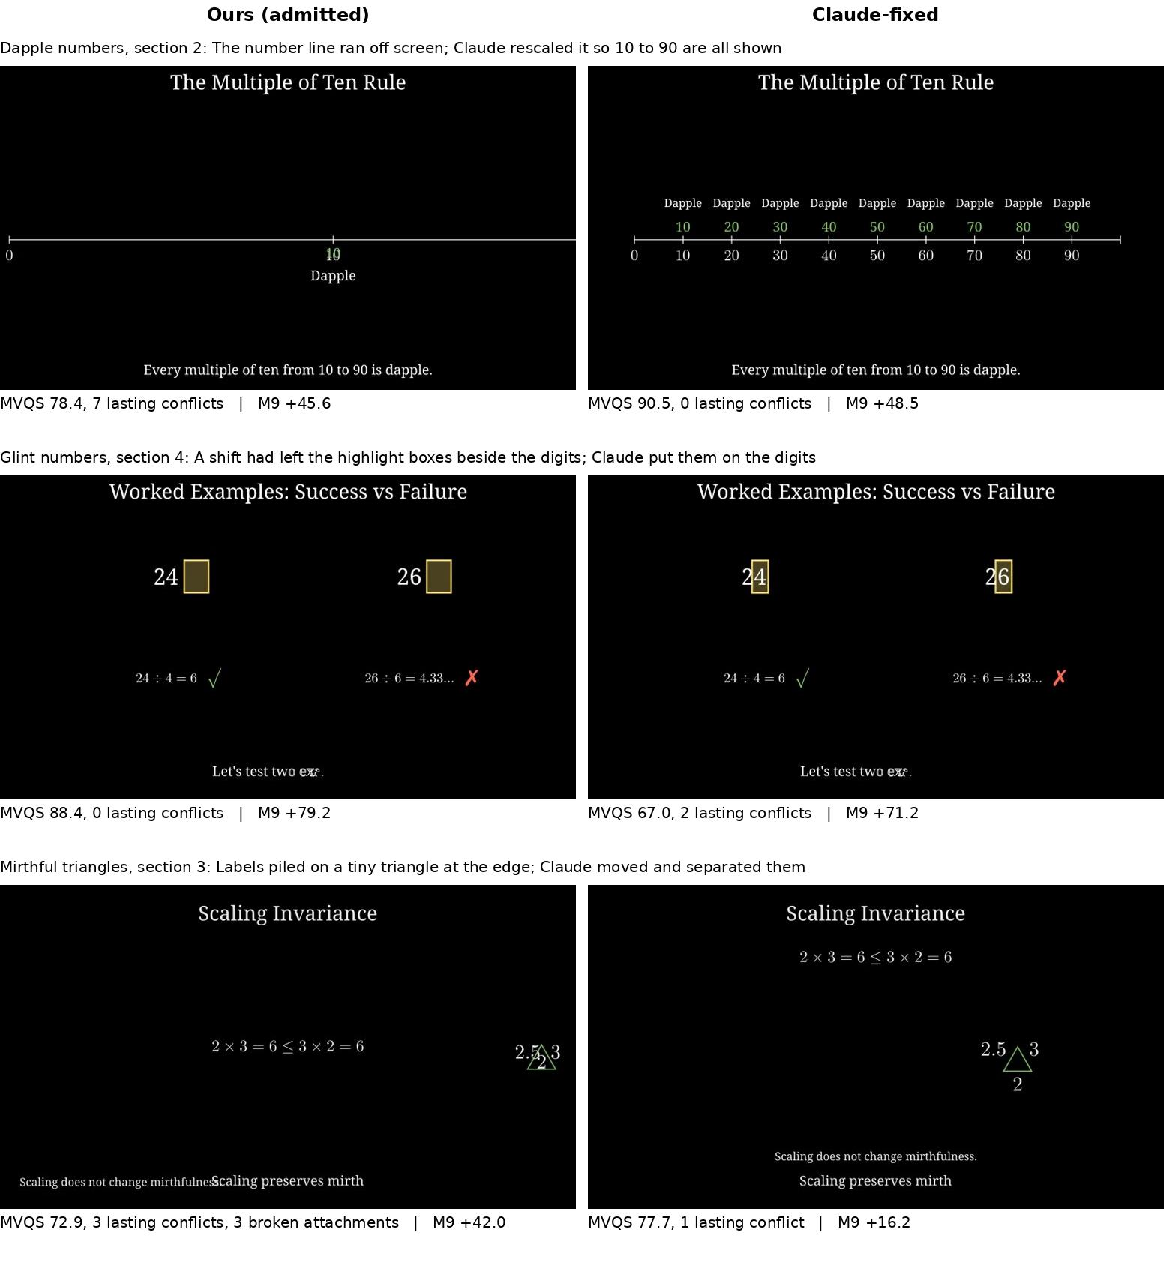
\includegraphics[width=\textwidth]{figures/layout_examples.pdf}
\caption{\textbf{The layout gets better; the score does not follow.} Three frames the student saw, from our admitted
video (left) and the Claude-fixed video (right). Under each frame: that section's layout score (MVQS), lasting
conflicts and broken attachments, then M9 for the whole concept (all four sections; \texttt{gemma4:26b}). Top: the
number line ran off screen and only 0 and 10 were visible. The fix shows 10 to 90, MVQS rises by 12 points, and M9
barely moves. Middle: a shift had left the highlight boxes over empty space beside the digits. The fix puts them on
the digits, which MVQS counts as two conflicts, so MVQS falls by 21 points although the frame is clearer. Bottom: labels
piled on a tiny triangle at the edge, and two captions collided. The fix separates them; MVQS rises a little, and M9
falls by 26 points. No single concept's change in M9 is beyond noise (Section~\ref{sec:results}).}
\label{fig:layout_examples}
\end{figure*}

\paragraph{Pipeline ablation} (Table~\ref{tab:stages}). All six stages (\S\ref{sec:ablation}) are scored on the
admitted NOVEL-12 concepts. The first stage, F0, is the pilot's loop. Its learner repair scores \NMRepair{} points of
M9 above the base video, ahead on \NMRepairPos{} of \NMRepairN{} concepts, and \NMRepairGeneric{} points above the
generic repair of the same size. Neither difference is beyond noise. Four insights follow from the later stages.
(i) \textbf{No feature makes the student's answers count.} By the rule fixed in advance, a feature helps if it
raises the learner repair's lead over the generic repair. From F1 to F5 that lead is \NMStageOneGeneric{},
\NMStageTwoGeneric{}, \NMStageThreeGeneric{}, \NMStageFourGeneric{} and \NMStageFiveGeneric{} points, against
\NMRepairGeneric{} at F0. Finding the weak section (F3) also does not beat rewriting every section beyond noise.
(ii) \textbf{The enforced gate keeps few revisions.} From F1 on, a revision that fails the gate is not used, and TEST
sees the base video instead. The gate kept the learner revision on only 1 to 5 of the 10 concepts per stage. So most
of each stage's learner videos are the base video.
(iii) \textbf{Kept revisions help on the 3 frames, not on the dense video.} The learner repair scores
\NMStageOne{}, \NMStageTwo{}, \NMStageThree{}, \NMStageFour{} and \NMStageFive{} points of M9 above the base video at
F1 to F5. Of the 17 revisions the gate kept, 16 raised M9. On the dense video (M7), the learner repair is at or below
the base video at every stage. Some gains rest on very little: on \emph{Tovan sums}, every kept revision fixes the same
single answer.
% Hand-counted from bench/results/noise-model/report.json (R1..R5, non-zero per-topic values: 17, of which 16 > 0);
% M7 learner - base and the edit sizes from bench/results/novel12-stages/report.md.
(iv) \textbf{None of these differences is beyond noise.} Four pass the question-swap test: F2, F3 and F5 against
the base video, and F5 against the generic repair. None holds across concepts, and none can: that test needs at least
six concepts to change in the same direction, and the gate let at most five change. Allowing for the ten stage
comparisons, none passes the question-swap test either. F3's difference comes from a single concept.
Two features do what they were built for. Checking the code before rendering (F2) raised the rewritten sections that
rendered from 25 to 28 of 32. Small edits (F5) change about 23\% of a section's lines, against about 70\% for the
rewrites of F2--F4. The edits did not keep the layout clean, though. The gate lets a revision lower the layout
score by up to 5 points and checks nothing else about the layout. In \RLWorse{} of the \RLRevisions{} revisions the F5 gate kept, the
edit added lasting conflicts or broken attachments. Over these \RLRevisions{}, lasting conflicts rose from
\RLConflictsBase{} to \RLConflictsLearner{} and broken attachments from \RLAttachBase{} to \RLAttachLearner{}
(\texttt{bench/repair\_layout.py}). So on NOVEL-12, with this student, the repair loop gives no gain
beyond noise at any stage. With ten concepts and most revisions refused, small benefits could not have been detected.

\begin{table*}[!tbp]\centering\small
\caption{Effect of each pipeline feature on NOVEL-12. Features are added one at a time; the base video is the same in every row. Gain: share of what the student did not know that it learned from 3 frames per section (version M9), in points. Learner $-$ generic: the learner repair against an equally large repair without the student's signal, scored on 3 frames (M9) and on the dense video (M7); small numbers: change against the row above. Layout: MVQS of the learner videos. Rewritten: sections rewritten and rendered. Used: topics whose final video is the revision.}\label{tab:stages}
\begin{tabular}{lrrrrrrrrr}\toprule & \multicolumn{4}{c}{Gain ($\uparrow$)} & \multicolumn{2}{c}{Learner $-$ generic ($\uparrow$)} & & & \\
\cmidrule(lr){2-5}\cmidrule(lr){6-7}
Stage & Base & Generic & Every section & Learner & 3 frames & Dense & Layout ($\uparrow$) & Rewritten & Used\\\midrule
F0: pilot loop & 42.4 & 42.4 & 38.9 & 48.5 & +6.1 & +3.4 & 81.3 & 25 & 10/10 \\
+ keep only revisions that pass the check & 42.4 & 44.5 & 45.2 & 50.2 & +5.6\worse{$-$0.5} & $-$3.7 & 84.5 & 25 & 5/10 \\
+ check the code before rendering & 42.4 & 51.2 & 42.2 & 54.6 & +3.4\worse{$-$2.2} & $-$5.4 & 84.2 & 28 & 4/10 \\
+ find the weak section like a debugger & 42.4 & 43.7 & 43.4 & 45.9 & +2.1\worse{$-$1.3} & $-$3.0 & 84.9 & 10 & 1/10 \\
+ block fixes that copy the practice quiz & 42.4 & 42.9 & 46.3 & 44.9 & +2.0\worse{$-$0.1} & $-$1.4 & 84.3 & 8 & 3/10 \\
+ small edits instead of rewrites & 42.4 & 42.2 & 42.8 & 48.5 & +6.3\better{+4.3} & $-$4.1 & 84.4 & 9 & 4/10 \\
\bottomrule\end{tabular}
\end{table*}


\section{Limitations}

\begin{itemize}
  \item \textbf{Local students see frames, not video.} The student receives up to 4 frames per second at 512 pixels
  (about 70 tokens a frame), without audio. Code2Video's own protocol (Gemini on the mp4) is implemented and exported
  for grading by hand, but not run.
  \item \textbf{Few students.} The main student is \texttt{gemma4:26b}; the prior was also measured with
  \texttt{qwen2.5vl:7b}. On NOVEL-12 we also asked Claude Haiku 5.5 and Sonnet 5.5, and they agree with
  \texttt{gemma4:26b} on the three findings we tested: the videos teach, the student learns the video's own topic,
  and the Claude fixes give no gain beyond noise. But Claude also wrote the questions and made the layout fixes, and it returns
  no log-probabilities, so its answers are scored right or wrong. Open students of other families are untested.
  \item \textbf{Invented concepts are small.} NOVEL-12's concepts are definable on one card; they test whether a video
  transmits a definition and its consequences, not deep understanding of a large theory. TEST was written by one model
  (Claude) and not reviewed by teachers.
  \item \textbf{The evidence judge is not calibrated.} Its decisions have not been compared with human annotations
  (e.g. Cohen's $\kappa$~\cite{cohen1960}); the forced-choice versions do not use it.
  \item \textbf{Twelve topics per set.} Means over 12 topics move a lot with one topic. We do not pool questions
  across topics, because the topic, not the question, is what receives a repair; a larger set would make the means
  steadier.
  \item \textbf{The local coder.} After one retry, two of twelve NOVEL-12 videos were still incomplete and only
  \AdmClean{} of \AdmTotal{} were clean. Stronger code models are future work; the Claude-fixed versions show the
  room.
  \item \textbf{The repair study is small.} All six stages are scored, on 10 concepts with one student. From F1 on,
  the gate kept the learner revision on at most half of them. A gain beyond noise across concepts was therefore out of
  reach, and small benefits of the repair remain possible. The two measures also disagree: kept revisions raise the
  gain on 3 frames (M9) but not on the dense video (M7).
  \item \textbf{The model-free checks are narrow.} The timing check covers two kinds of fault; the attachment check
  skips labels anchored to a text glyph.
  % Hand-typed from bench/layout_study.log, layout_study_rerun.log, layout_study_attach.log (sum of 'conflicts'), and
  % from bench/results/layout-study/rows.json of 22:33 (fixed tracker, commit 937336d), summed over the 10 admitted concepts.
  \item \textbf{The conflict counts were measured with a tracker bug.} The tracker sometimes gave a deleted object's
  code line to a new one, so the same code gave 29, 29 and 31 lasting conflicts on three runs. With the bug fixed,
  the counts repeat exactly. Our videos then have 27 lasting conflicts, as do our videos with timing fixes, against 4
  for the Claude-fixed versions. The tables keep the earlier counts. MVQS, the attachment counts and every
  conclusion are unchanged.
  \item \textbf{Counterfactual relabelling was not applied to MMMC.} It would rewrite TEST per video and break the
  paired design; NOVEL-12 controls the prior instead.
\end{itemize}

\section{Future work}

\begin{itemize}
  \item \textbf{A gate that sees what a viewer sees.} The repair gate checks only the layout score, and it let through
  revisions that added conflicts and broken attachments. A gate that also counts these faults is built (crowding,
  conflicts, attachments) but not yet evaluated.
  \item \textbf{A larger study.} With 10 concepts of 8 questions, only effects of about 24 points or more are
  detectable. More concepts, and a gate that keeps more revisions, would let smaller effects of layout and repair show.
  \item \textbf{Stronger coders and a fixed layout.} A study with Claude models as planner and coder, and with
  Code2Video's anchor-grid layout, was running at submission. It asks whether better code, rather than repair,
  is what makes videos teach more.
  \item \textbf{Students that watch video.} Code2Video's protocol (a model reading the mp4 with audio) is implemented
  but not run; open students of other families are untested.
  \item \textbf{A layout score that measures reading.} MVQS measures box separation. A score built on attachments, on
  what is on screen when, and on crowded text would track what a viewer can read.
  \item \textbf{Cheaper scoring.} The dense video is about two thirds of the student's work. Scoring on 3 frames per
  section only (M9) is implemented as an option, for studies that do not need M7.
\end{itemize}

\section{Conclusion}

TeachQuiz, as published and as we first ran it, could not have detected teaching: a grading bug dropped answers,
the student's refusals set $S_1$, and the questions were answered from prior knowledge. Forced choice, a measured
prior, normalisation, dense silent frames, a motion control, continuous scoring and option rotation each address a
named failure, and the ladder shows which of them a teaching metric actually needs. A benchmark whose prior is
controlled by construction is the precondition for asking whether a repair teaches. The layout score has the same
weakness from the other side: it measures box separation, not whether a viewer can read what belongs to what. On
NOVEL-12, the repair loop gives no gain beyond noise at any stage. None of the added features makes the student's
answers beat a repair of the same size made without them.


\bibliographystyle{plainnat}
\bibliography{refs}
\end{document}
